\documentclass[xcolor=dvipsnames]{beamer}
\usepackage{tikz}
\usepackage{url}
\usepackage{tabularx}
\usepackage{multirow}
\usecolortheme[named=Plum]{structure} 
\usetheme[height=7mm]{Rochester} 
\setbeamertemplate{navigation symbols}{} 
\title[Pacemaker modes]{Pacemaker Modes}

\newcommand {\framedgraphic}[2] {
    \begin{frame}{#1}
        \begin{center}
            \includegraphics[width=\textwidth,height=0.8\textheight,keepaspectratio]{#2}
        \end{center}
    \end{frame}
}

\begin{document}



  \begin{frame}
    \frametitle{Heart}
        \begin{center}
            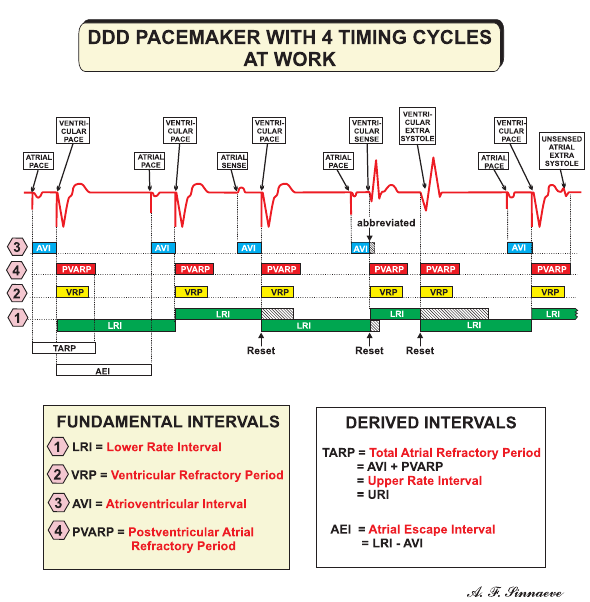
\includegraphics[width=\textwidth,height=0.8\textheight,keepaspectratio]{../Figures/intervals.png}
        \footnote{Cardiac Pacemakers Step by Step: An Illustrated Guide}
        \end{center}
  \end{frame}


  \begin{frame}{}
    \frametitle{Pacemaker modes}
    \begin{tabularx}{\textwidth}{|X|X|X|X|}
      \hline
              Chamber(s) Paced & Chamber(s) Sensed & Response To Sensing & Rate Modulation  \\ \hline
              0-None           & 0-None            & 0-None              & \multirow{2}{2cm}{R-Rate Modulation}  \\ % \hline
              A-Atrium         & A-Atrium          & T-Triggered         &                    \\ % \hline
              VV-Ventricle      & V-Ventricle       & I-Inhibited         &                    \\ % \hline
              D-Dual           & D-Dual            & D-Tracked           &                  \\
      \hline
    \end{tabularx}

  \end{frame}



    \framedgraphic{AOO}{../Modes/AOO.png}

    \framedgraphic{VOO}{../Modes/VOO.png}
    \framedgraphic{DOO}{../Modes/DOO.png}
    \framedgraphic{VVI}{../Modes/VVI.png}
    \framedgraphic{AAI}{../Modes/AAI.png}
    \framedgraphic{DDI}{../Modes/DDI.png}
  
\end{document}

